\chapter{Theory \& Design}\label{chapter:theory-and-design}
In this chapter, the theory and design for this project will be described and specified.
The theory will cover position calculation techniques, Bayesian networks, and normal distribution.
Afterwards, the machine intelligence theories of this project are specified, game and system design will be reviewed using event tables, state diagrams, and illustrated concepts.

%\section{Dead Reckoning}\label{section:theory-dead-reckoning}
%Dead-Reckoning \citep{thesis:dead-reckoning}, as previously described in \secref{section:dead-reckoning}, is a movement tracking technique. In the previous section the concept was described, whereas in this section it will be described thoroughly in regards to the mathematical details.
%
%%\subsection{Pedestrian Dead Reckoning}
This section is based on theory from \citep{misc:PedestrianDeadReckoningSystem}.
The pedestrian DR uses the accelerometer and the gyroscope to detect steps and estimate the step-length.
Steps can be detected in 3 different ways, peak detection, zero crossing detection, and flat zone detection.

Peak detection finds the maxima and minima of the accelerometer output, and when a maximum is found it looks for the next minimum which determines a step, and vice versa. 
Every step has acceleration phase followed by a deceleration phase, peak detection finds these two phases by finding a local maximum and minimum that are close to each other, as seen in \figref{figure:peak-detection}.

Zero crossing detection checks where the accelerometer output crosses the x axis, with the heuristic that a step has a minimum and a maximum duration. 
As a step has three crossings of the x axis, first one is where it starts to accelerate, second is when the acceleration stops and the deceleration begins, and third is when the deceleration stops and the step is finished. 
These three crossings can be seen in \figref{figure:zero-crossing}.

Flat zone detection constrains the user to stop in between each step, and find the flat zones in the graph.
A flat zone is a zone on the graph where oscillation is not large enough to be included as a step.\fxnote{mangler nogle passende maalinger til den her som har pauser ind i mellem hvert skridt.}
\begin{figure}[H]
\centering
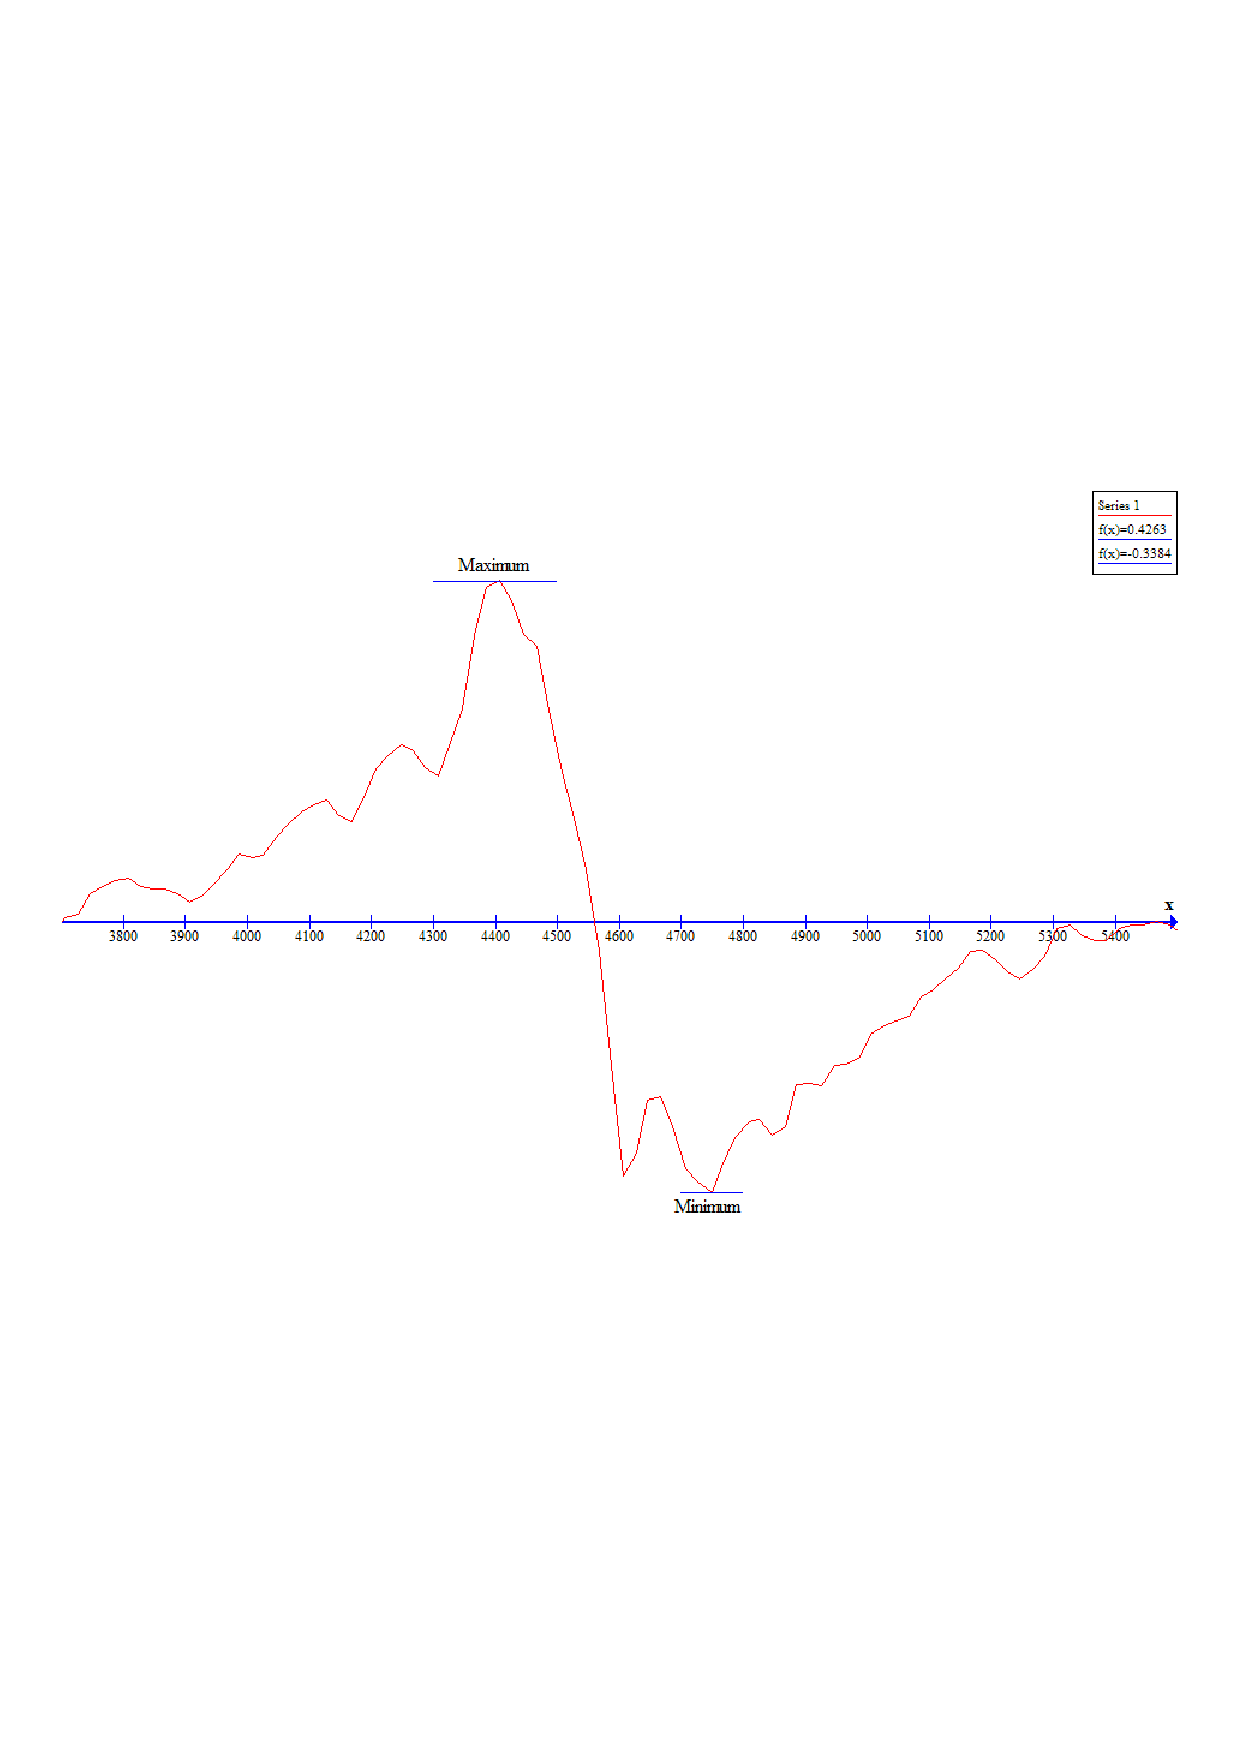
\includegraphics[trim=0 8cm 0cm 8cm, clip,scale=0.5]{media/peak-detection}
\caption{Peak detection finding one step.}
\label{figure:peak-detection}
\end{figure}

\begin{figure}[H]
\centering
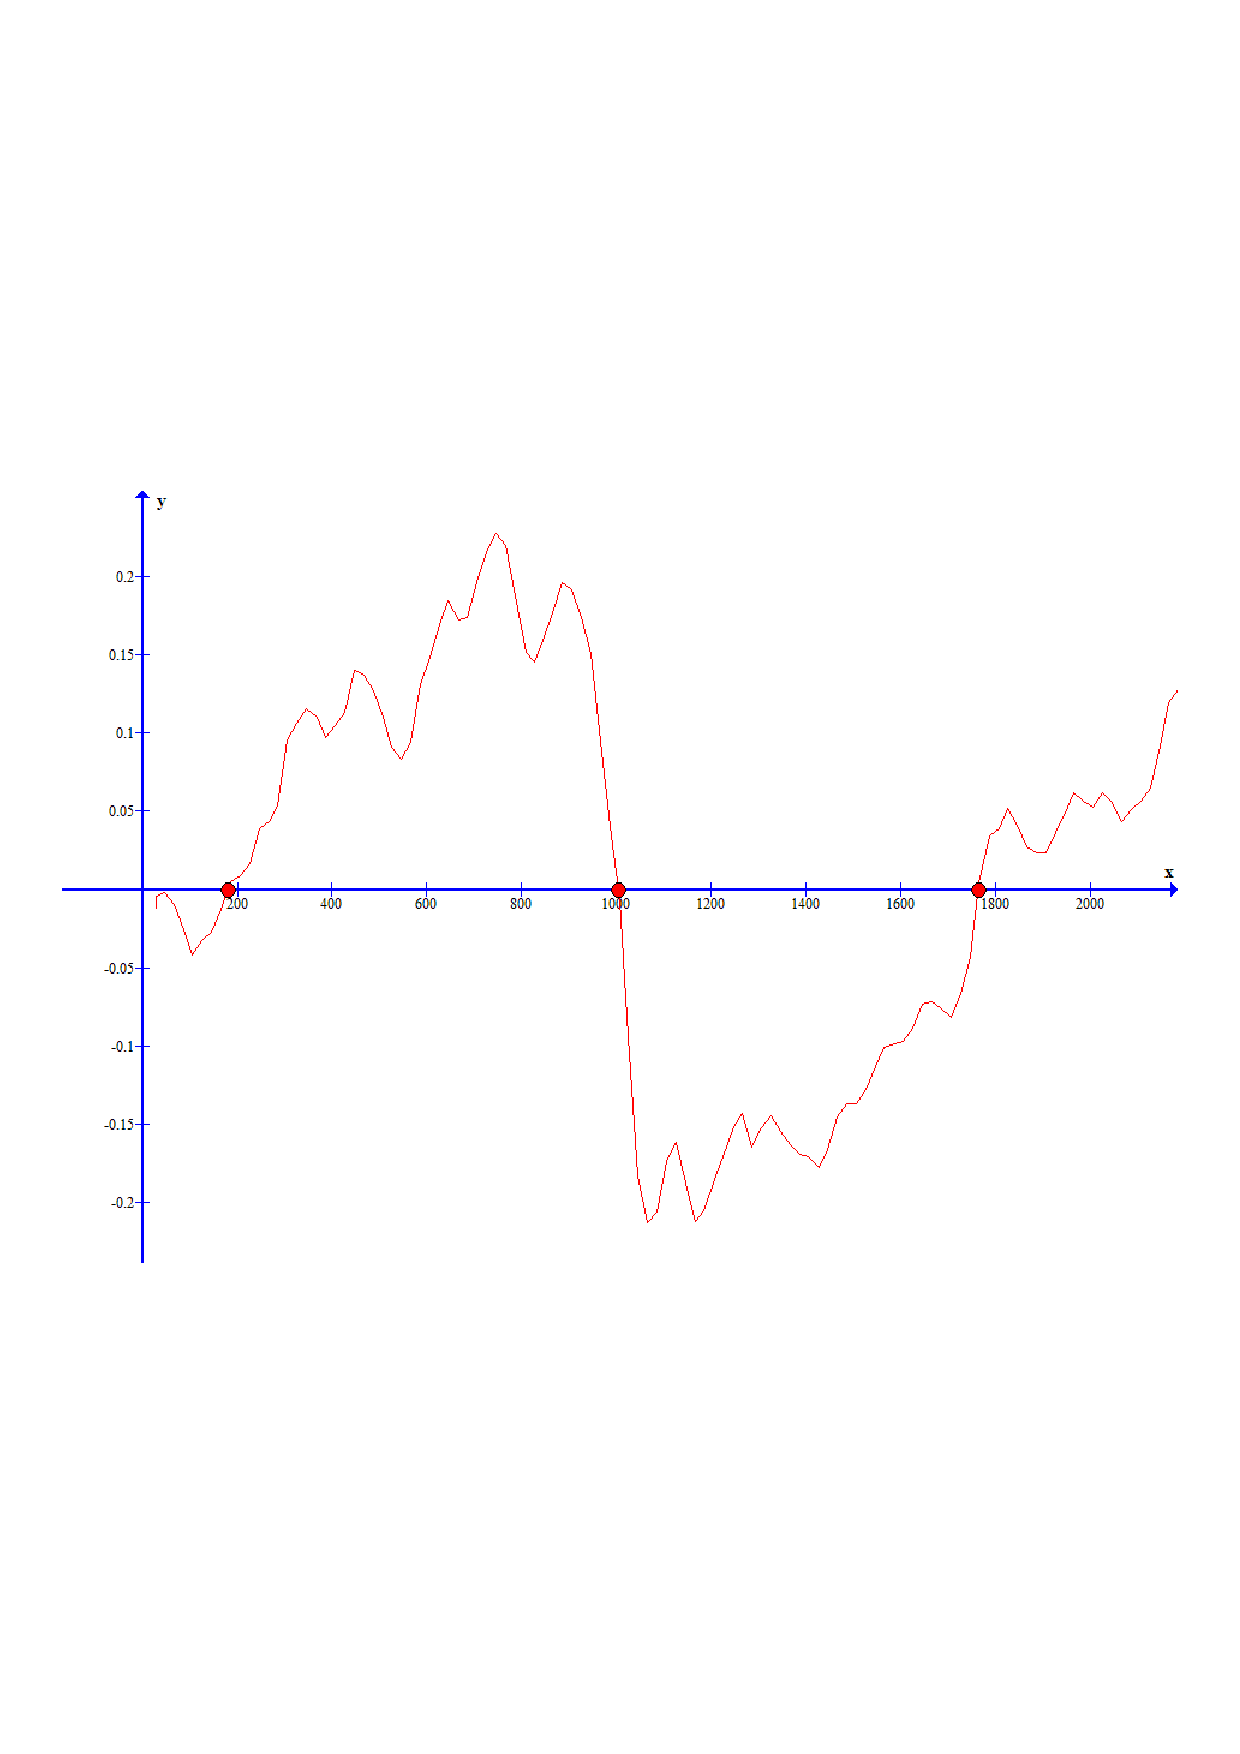
\includegraphics[trim=0 8cm 0cm 8cm, clip,scale=0.5]{media/zero-crossing}
\caption{Zero crossing determining a step.}
\label{figure:zero-crossing}
\end{figure}

After finding the step, the step length can be determined by a linear combination of walking velocity and variance of the accelerometer, \eqref{eq:steplength}. \fxnote{er usikre på denne formel, vi mener v er noise fra accelerometer men er ikke sikker}
The walking distance, \eqref{eq:walkingdistance}, is the accumulated value of all the steps, which were found using the previously described algorithms and the step length equation.
\begin{equation}\label{eq:steplength}
	Step length = \alpha * f + \beta * v + \gamma \\
\end{equation}
\begin{equation}\label{eq:walkingdistance}
	Walking distance = \sum\limits_{i=1}^{n} (\alpha * f_i + \beta * v_i + \gamma)
\end{equation}
where,
\begin{itemize}
	\item[$\alpha , \beta$] is weights of walking parameters.
	\item[$\gamma$] is a constant.
	\item[$f_i$] is the walking velocity of the i-th step.
	\item[$v_i$] is the acceleration variance of the i-th step.
\end{itemize}

These formulas can be erroneous as the location of the phone can change which creates bad inputs in the calculation of the walking distance.
Determining the location of the phone is therefore important in pedestrian dead reckoning i.e if it is in the pocket, bag, or hand. But as this project is constraint to having the phone in a fixed position, phone location awareness as it is not necessary.

\section{Position Calculations}\label{sec:position-calculations}
In order to develop a game where a user moves to control the game, it is necessary to register these movements and calculate a position. 
Calculating positions can be done by analysing the data given from the accelerometer in the phone.
The output of the accelerometer is the accelerations of the three axis' of the accelerometer.
\figref{figure:acceleration-chart} and \figref{figure:velocity-chart} shows two graphs with each graph showing three steps.
\figref{figure:acceleration-chart} is the acceleration along the y-axis of the phone. 
\figref{figure:velocity-chart} is the velocity along the y-axis of the phone.
The velocity is calculated by taking the integral of the acceleration, the formula is as follows:
\begin{equation*}
v(T) = \int_0^T \! a(t) \, \mathrm{d}t
\end{equation*} 
where, $v(T)$ is the velocity at time $T$, and $a(t)$ is the acceleration at time $t$.

A graph with accelerations and a graph with the corresponding velocities can be seen in \figref{figure:acceleration-chart} and \figref{figure:velocity-chart}, respectively.

\begin{figure}[H]
	\centering	
	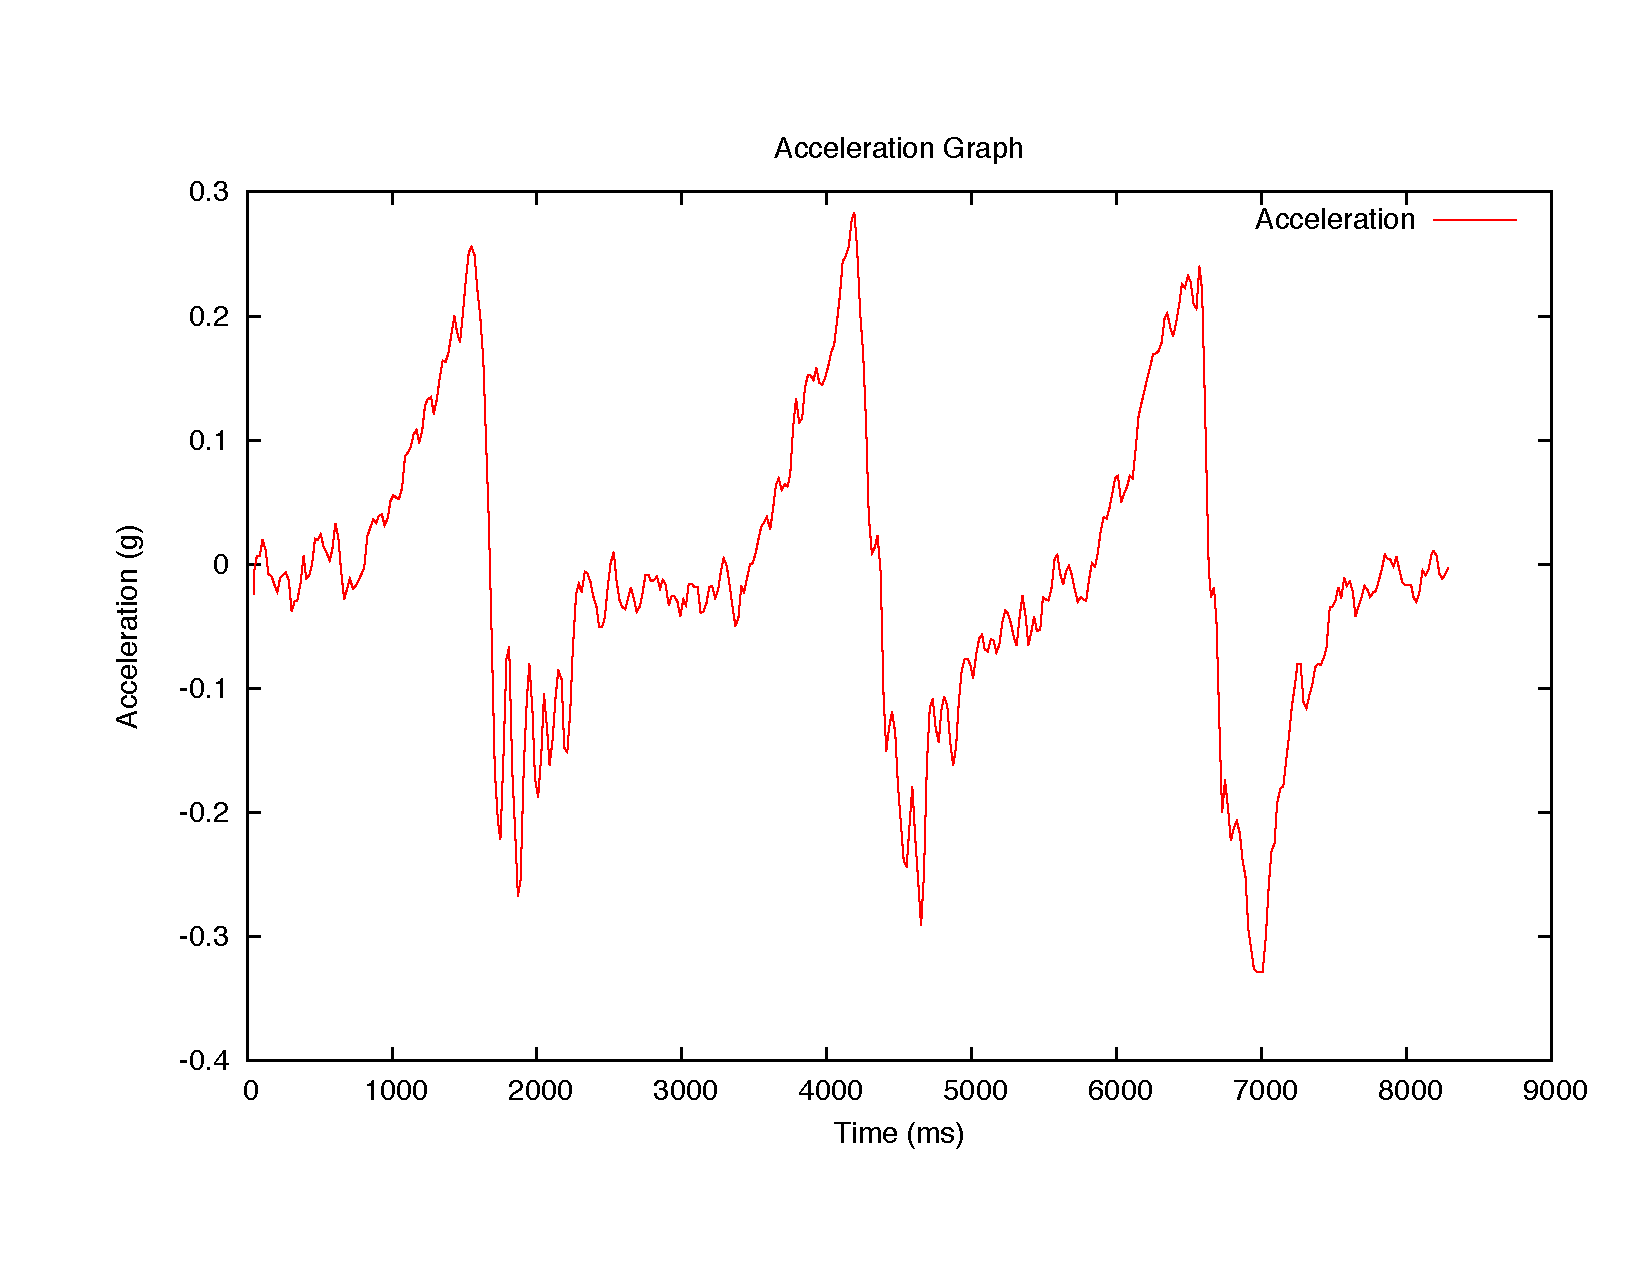
\includegraphics[scale=0.4, trim=0cm 2cm 0cm 2cm]{media/gnuplot/acceleration.pdf}
	\caption{Acceleration readings over three steps.}
	\label{figure:acceleration-chart}
\end{figure}

\begin{figure}[H]
	\centering	
	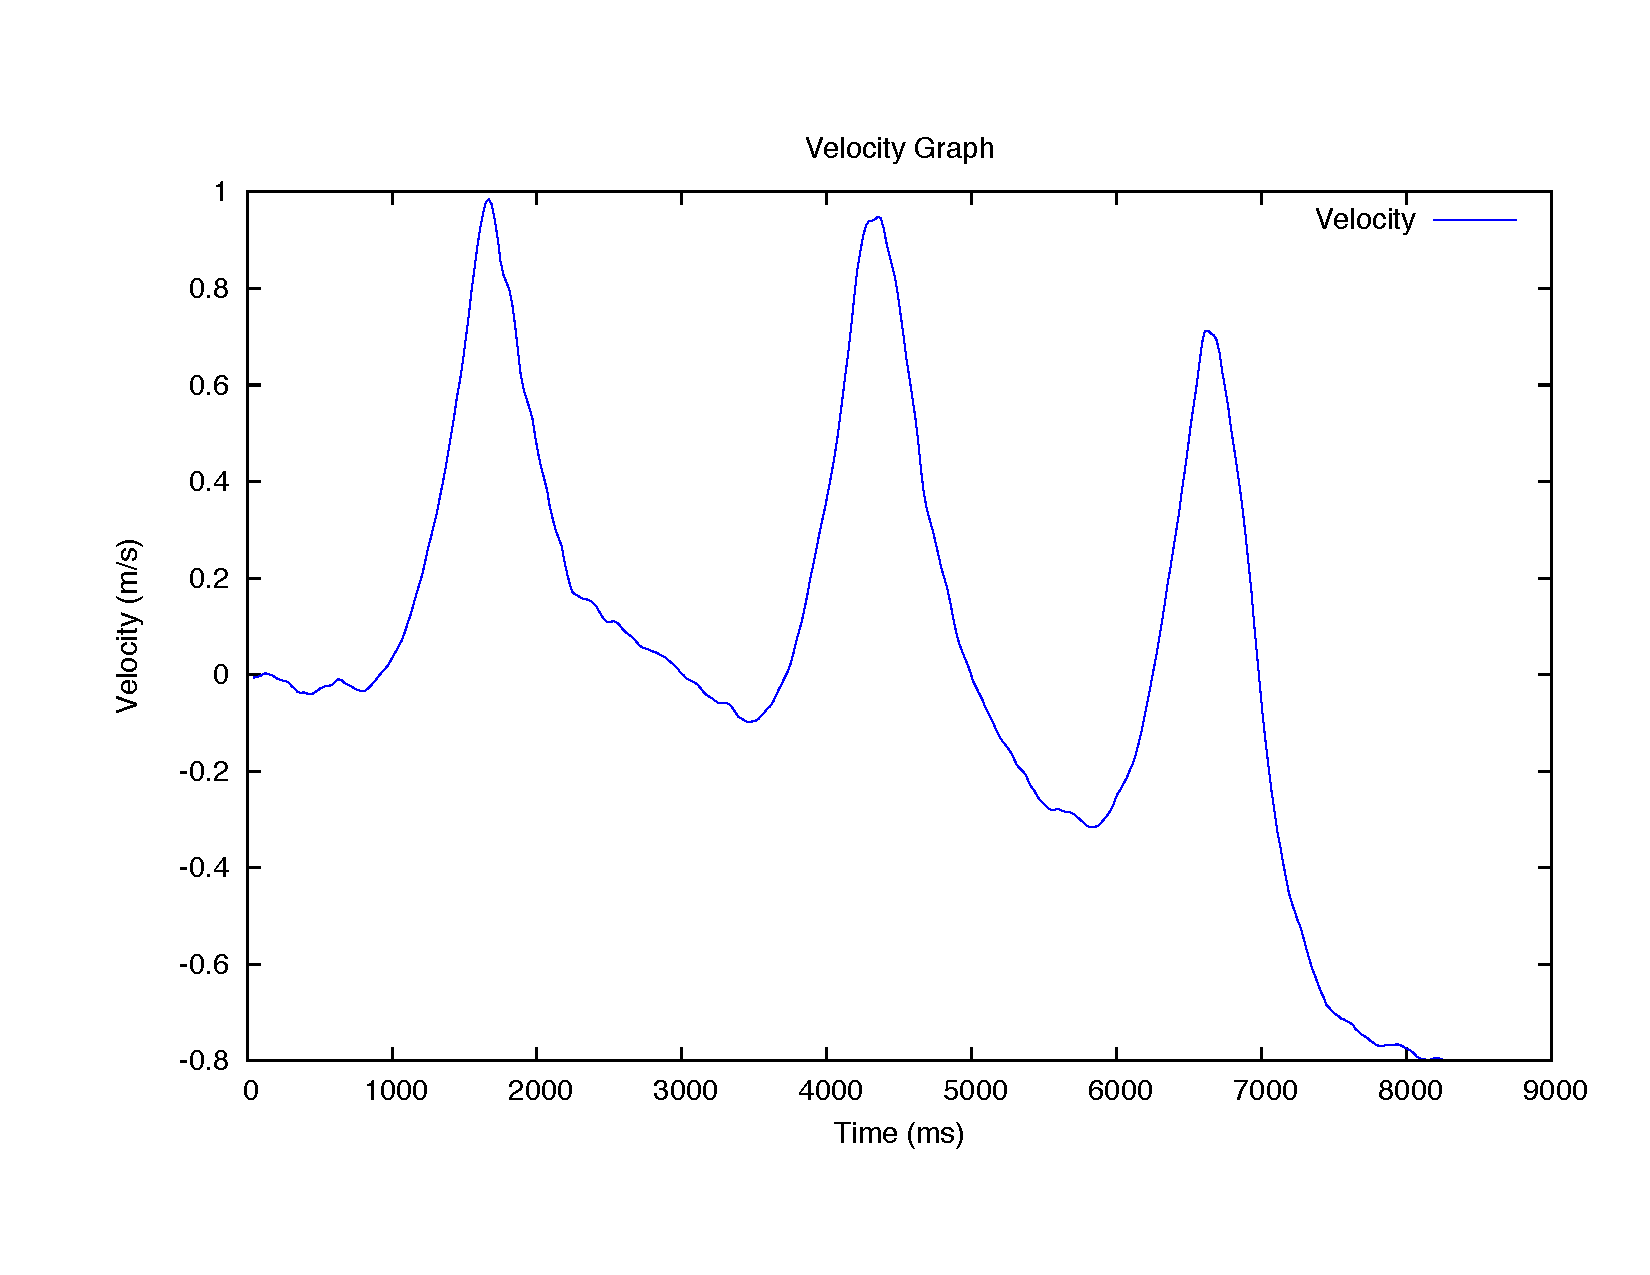
\includegraphics[scale=0.4, trim=0cm 2cm 0cm 2cm]{media/gnuplot/velocity.pdf}
	\caption{Velocity calculations over three steps.}
	\label{figure:velocity-chart}
\end{figure}

The velocity graph is smoother than the acceleration graph because each point on the velocity graph is a summation of the area of the acceleration graph.

To determine the position, the area under the velocity graph is calculated by taking the integral of the velocity over time, as seen in the following equation:

\begin{equation}\label{eq:integral-velocity}
     s(T) = \int_0^T v(t)\mathrm{d}t 
\end{equation}
where, $s(T)$ is the distance at time $T$, and $v(t)$ is the velocity at time $t$. 

The value can be used in conjunction with the previous position to calculate an approximation of the new position.
The actual values can be observed by video footages of people sidestepping with the phone.
As seen in the graphs, noise exists and should be corrected by use of filters.
%step detection
%step-length estimation
%Phone location awareness
%
%Calculate the double integration:
%accelerometer -> velocity -> step-length.

%teknikker til DR
%beregner skridt ud fra velocity.
%augument inertial/magnetic sensor (IMMU)
%Pedestrian 


%implementations teknikker
%http://www.diydrones.com/profiles/blogs/a-simple-deadreckoning
%http://www.gamasutra.com/view/feature/3230/dead_reckoning_latency_hiding_for_.php
%http://www.mmorpg.com/discussion2.cfm/post/2228522#2228522
%http://stackoverflow.com/questions/1261119/how-to-implement-dead-reckoning-when-turning-is-involved
%http://www.comp.lancs.ac.uk/~kristof/research/notes/deadreck/deadreck.html
%Direction

%Length

%Noise

%Extended Kalman Filter

%DRA-1
\section{Position Calculations}\label{sec:position-calculations}
In order to develop a game where a user moves to control the game, it is necessary to register these movements and calculate a position. 
Calculating positions can be done by analysing the data given from the accelerometer in the phone.
The output of the accelerometer is the accelerations of the three axis' of the accelerometer.
\figref{figure:acceleration-chart} and \figref{figure:velocity-chart} shows two graphs with each graph showing three steps.
\figref{figure:acceleration-chart} is the acceleration along the y-axis of the phone. 
\figref{figure:velocity-chart} is the velocity along the y-axis of the phone.
The velocity is calculated by taking the integral of the acceleration, the formula is as follows:
\begin{equation*}
v(T) = \int_0^T \! a(t) \, \mathrm{d}t
\end{equation*} 
where, $v(T)$ is the velocity at time $T$, and $a(t)$ is the acceleration at time $t$.

A graph with accelerations and a graph with the corresponding velocities can be seen in \figref{figure:acceleration-chart} and \figref{figure:velocity-chart}, respectively.

\begin{figure}[H]
	\centering	
	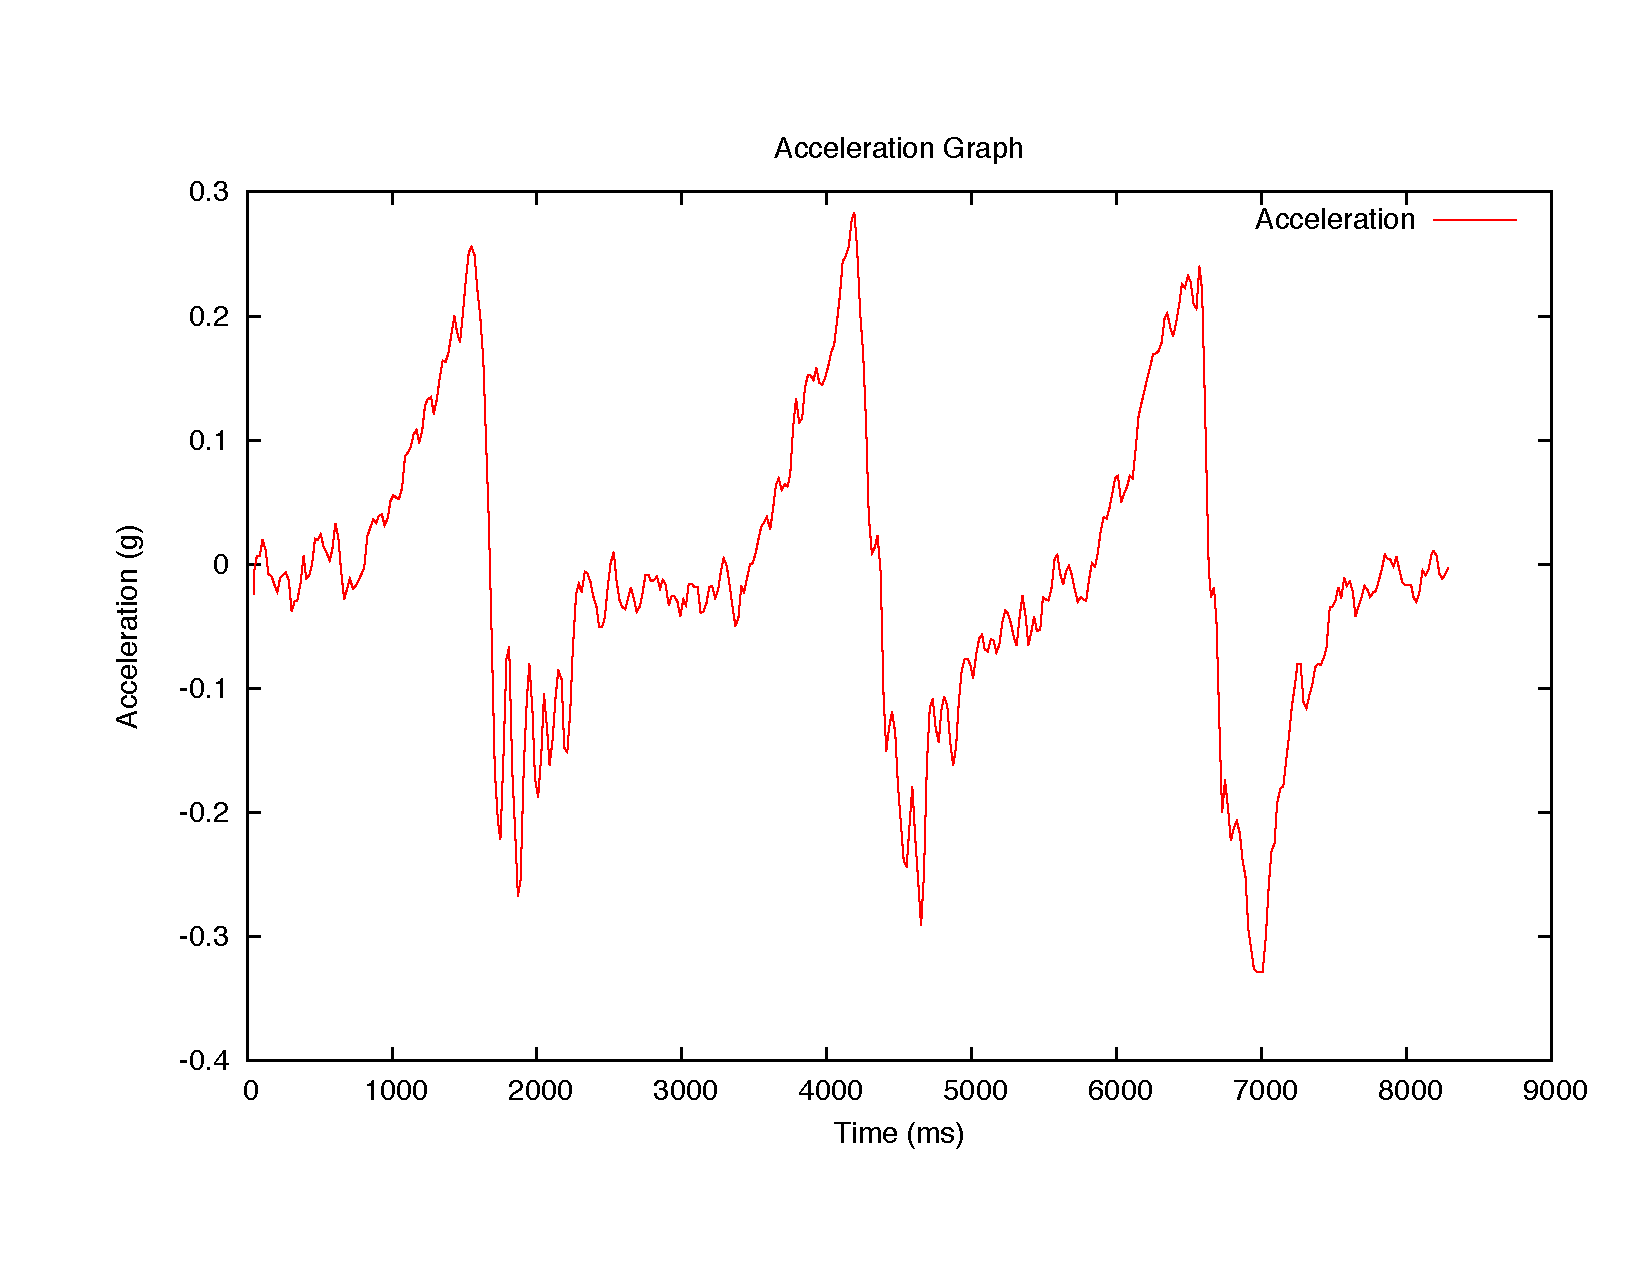
\includegraphics[scale=0.4, trim=0cm 2cm 0cm 2cm]{media/gnuplot/acceleration.pdf}
	\caption{Acceleration readings over three steps.}
	\label{figure:acceleration-chart}
\end{figure}

\begin{figure}[H]
	\centering	
	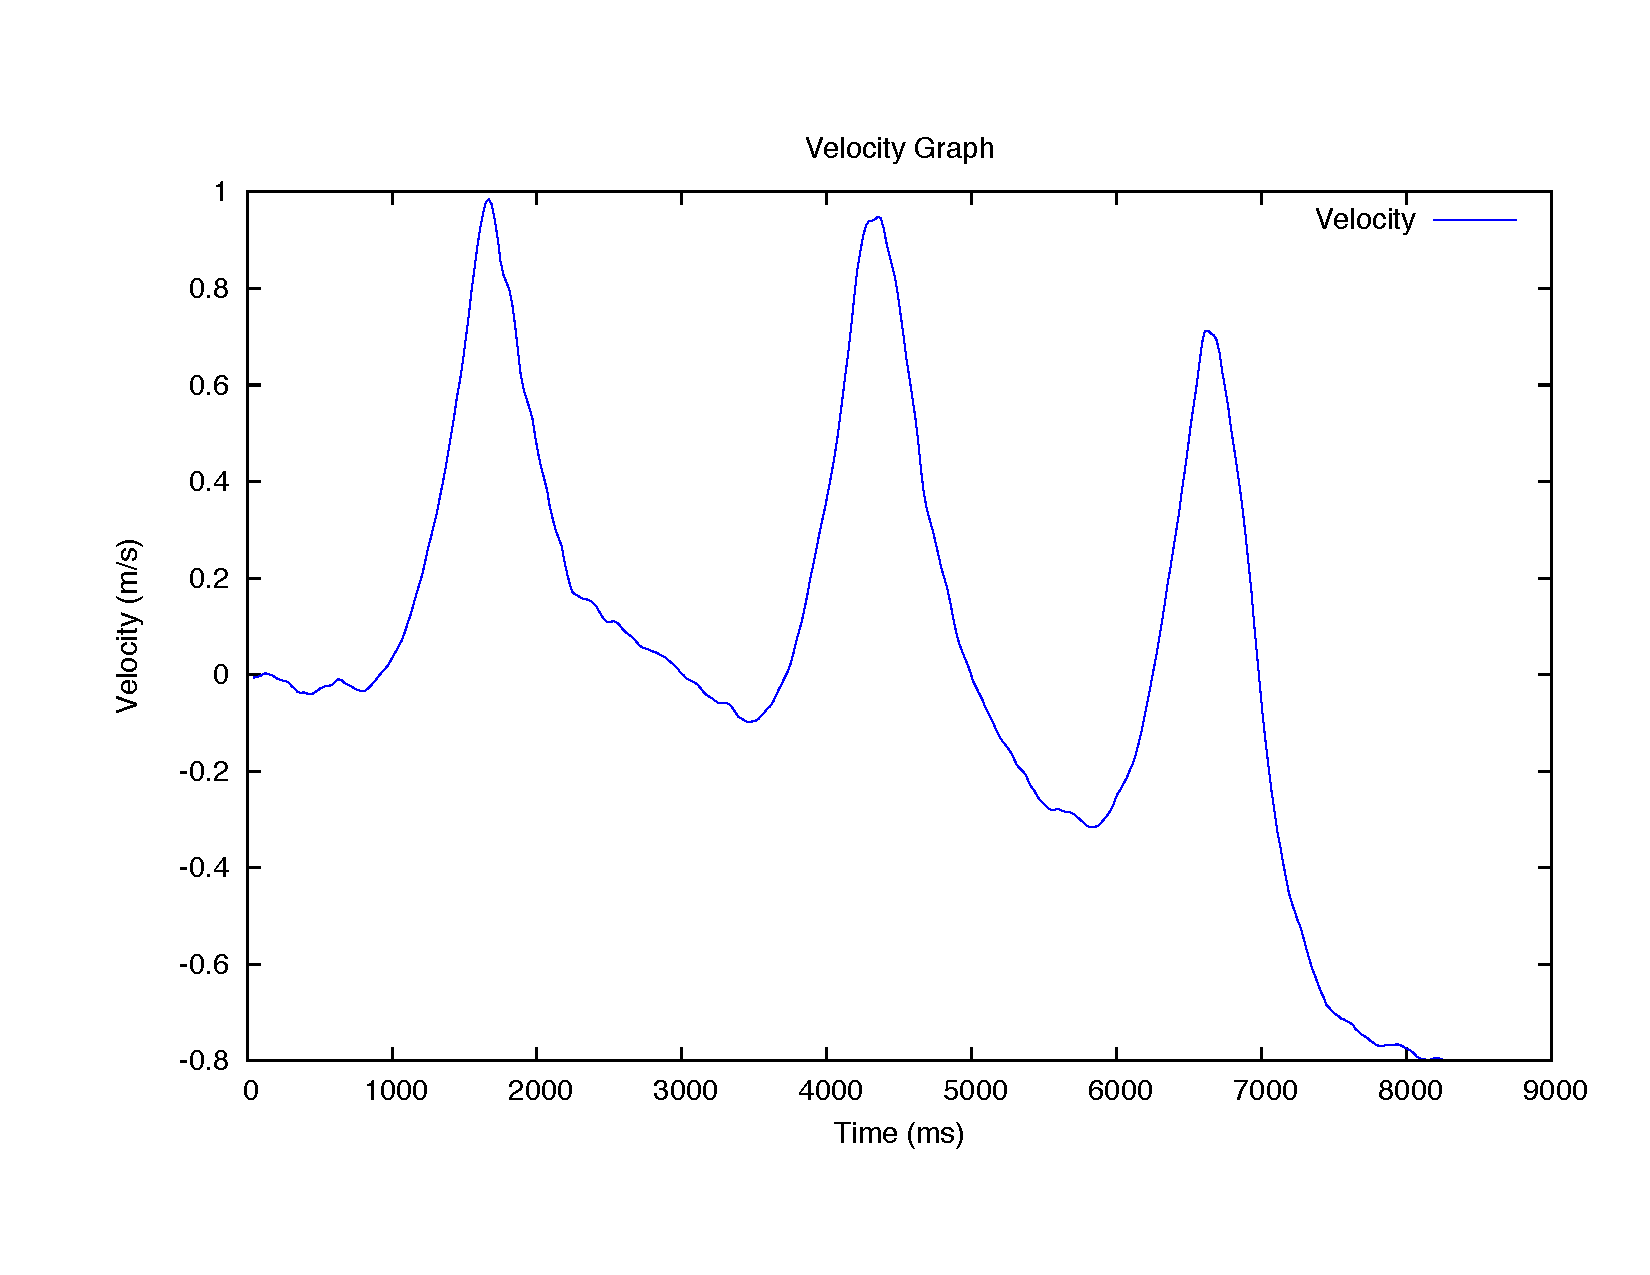
\includegraphics[scale=0.4, trim=0cm 2cm 0cm 2cm]{media/gnuplot/velocity.pdf}
	\caption{Velocity calculations over three steps.}
	\label{figure:velocity-chart}
\end{figure}

The velocity graph is smoother than the acceleration graph because each point on the velocity graph is a summation of the area of the acceleration graph.

To determine the position, the area under the velocity graph is calculated by taking the integral of the velocity over time, as seen in the following equation:

\begin{equation}\label{eq:integral-velocity}
     s(T) = \int_0^T v(t)\mathrm{d}t 
\end{equation}
where, $s(T)$ is the distance at time $T$, and $v(t)$ is the velocity at time $t$. 

The value can be used in conjunction with the previous position to calculate an approximation of the new position.
The actual values can be observed by video footages of people sidestepping with the phone.
As seen in the graphs, noise exists and should be corrected by use of filters.
\section{Filters}\label{sec:filters}
Filters are needed to cancel out noise from the acceleration inputs.
Noise is caused by electronic noise from the circuitry and mechanical noise from the sensor itself \citep{misc:SensorsMag}.

\subsection{The Kalman Filter} 
%The theory from this section is based on \citet{electronic:KalmanGreg}.
The Kalman filter is built upon a simple found propagation in a dynamic Bayesian network, where the previous state and new observations is used to find the current state.
A Bayesian network can be used to find the probability distribution of the next state given the current state.
The Kalman filter is a linear dynamic system, which means the function derived will be a linear function.

The Kalman filter structure can be modelled as a dynamic Bayesian network, see \figref{fig:kalman-filter}.
Insertion of evidence in the network will be described in \secref{section:insert-evidence}.
Additional theory for Kalman filters exists, but has not been examined, as it was unnecessary for this project.
\begin{figure}[H]
	\centering
	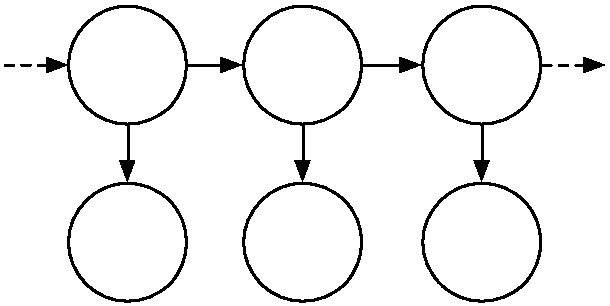
\includegraphics[scale=0.6]{media/kalman-filter}
	\caption{The Kalman filter.}
	\label{fig:kalman-filter}
\end{figure}

\begin{comment}
The state equation is:
\begin{equation*}
	 \textbf{x}_{k} = \textbf{F}_{k} \textbf{x}_{k-1} + \textbf{B}_{k} \textbf{u}_{k-1} + \textbf{W}_{k-1}
\end{equation*}
where
\begin{itemize}
	\item[$x_k$] is a state matrix at state $k$.
	\item[$F_k$] is the state transition matrix that is applied to the previous state matrix $x_{k-1}$.
	\item[$B_k$] is the transition matrix from the previous state $u_{k-1}$.
	\item[$W_k$] is the noise gained from the previous states, also called Guassian noise.
\end{itemize}


The previous state can also include noise, because of uncertainty of the measurement, and thus do not have an accurate value, this must therefore be taken into account.
To find the previous state measurement value, a linear function combining the sensor value and the measurement noise is used.
\end{comment}

\subsection{Exponential Moving Average}
\label{subsection:exponential-moving-average}
The exponential moving average (EMA) reduces noise from the input and smoothes the data set.
The formula for exponential moving average is as follows:
\begin{equation*}
	EMA_i = \alpha * y_i + (1-\alpha) * EMA_{i-1}
\end{equation*}
where,
\begin{itemize}
	\item[]
	\begin{itemize}
		\item[$EMA_i$] is the exponential moving average value for the i'th data element.
		\item[$\alpha$] is a coefficient which determines the smoothness of the data.
		\item[$y_i$] is the i'th observed value.
	\end{itemize}
\end{itemize}
$EMA_i$ is calculated recursively, updating the values. 
The previously observed values are accounted for in the formula by $EMA_{i-1}$ but their impact is reduced in each step.
The formula works by weighing the new value and adding it with the weighted previously observed values $EMA_{i-1}$.
\figref{fig:EMA} shows two graphs where the red graph is the raw data and green is the data after running the exponential moving average, with an $\alpha$ of $0.1$.

\begin{figure}[H]
	\centering
	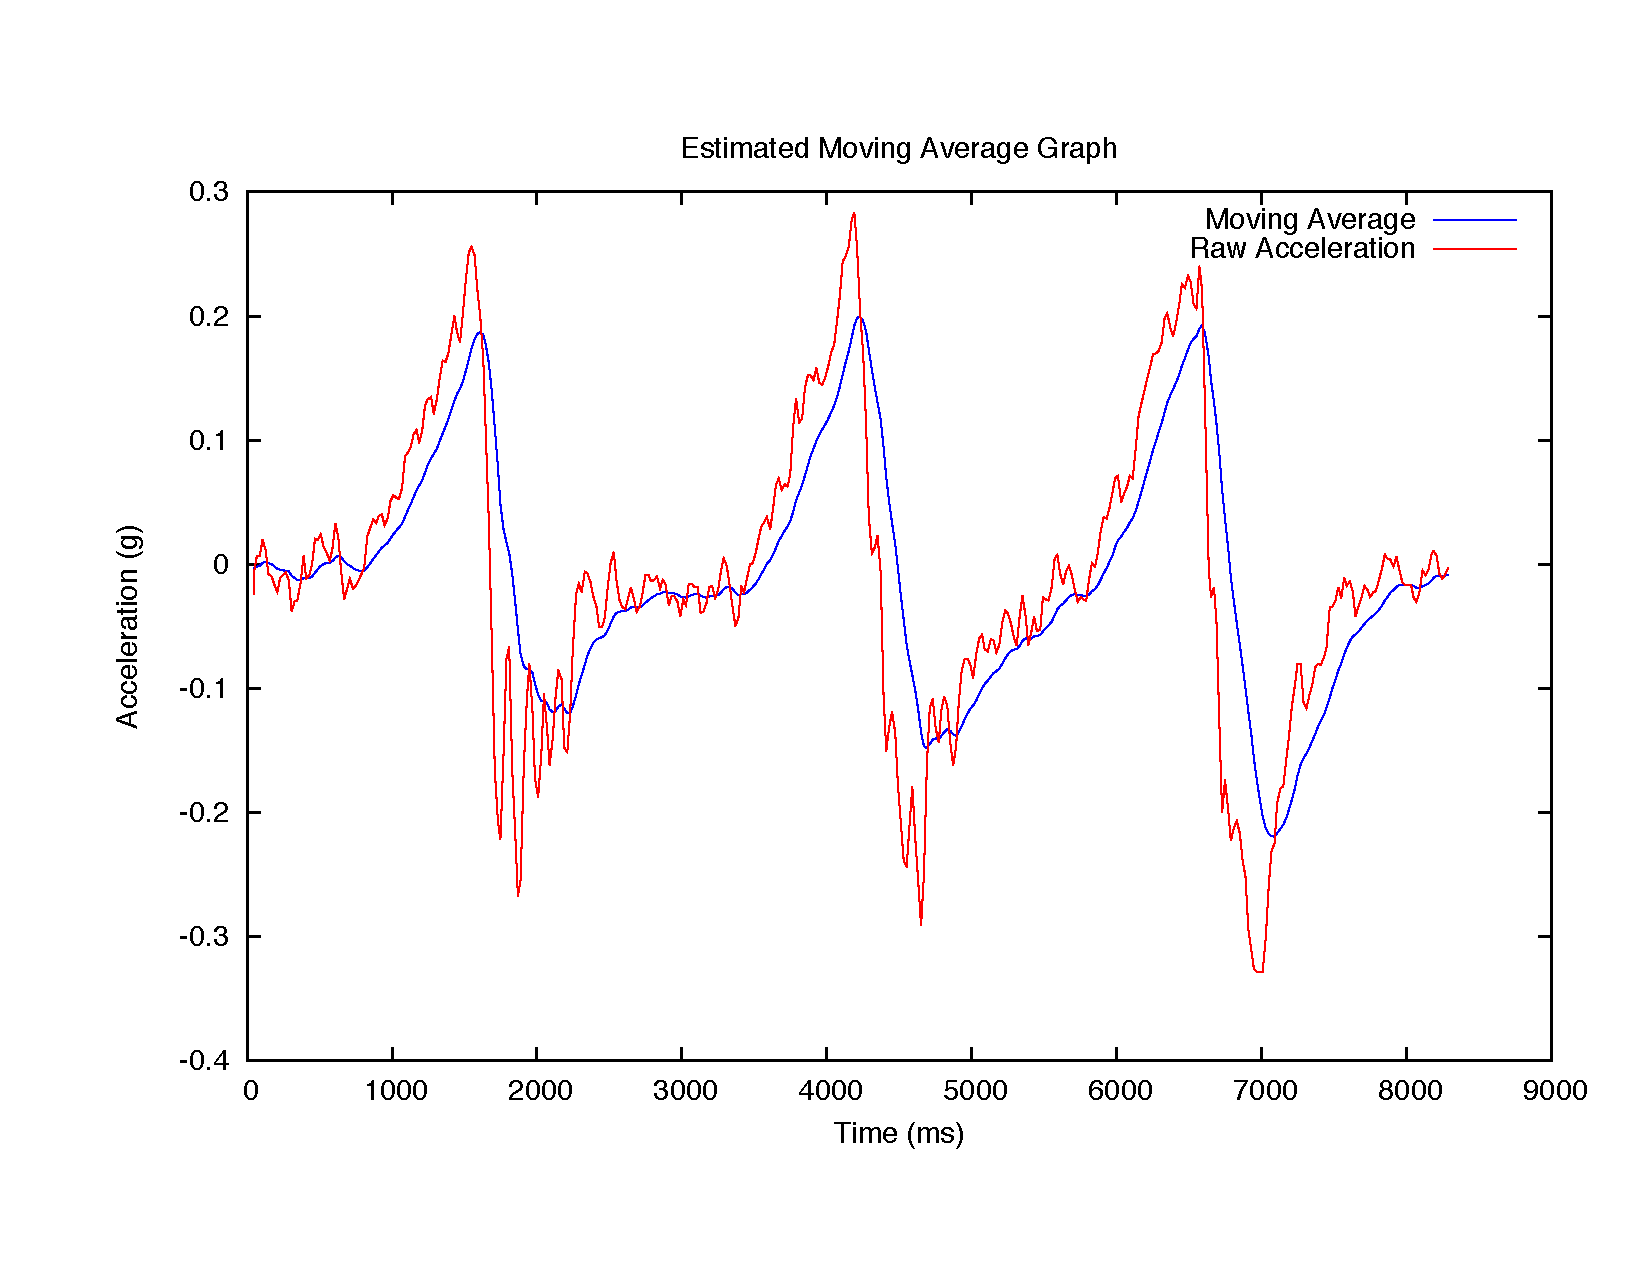
\includegraphics[scale=0.45, trim=0cm 2cm 0cm 2cm]{media/gnuplot/ema.pdf}
	\caption{Raw data, red graph, compared with the EMA data, blue graph.}
	\label{fig:EMA}
\end{figure}

\section{Bayesian Network}\label{section:bayesian-network}
A Bayesian network is a directed acyclic graph, where each edge shows how a parent has an influence on its child.
The Bayesian network, see \figref{figure:simple-Bayesian-network}, shows how the different variables affect each other.
In the figure there are three different types of variables.
The first variable $A$, which is shaded, is an information variable. 
Information variables, can be either stochastic or deterministic, hold information that are obtained from input-sources.
The second variable $B$ is a deterministic variable, marked with two circles, the data in this variable type is based on parent values, and has no probability distribution.
Lastly, the variable $C$ with a single circle, is called a stochastic variable. 
Stochastic variables can be either continuous or discrete.
Continuous variables can hold an infinite number of values between two points, while discrete is a finite set.
As an example, a continuous variable holding a value between two points, 0 and 1, can have any number between these two points, which is an infinite set of real numbers.

\begin{figure}[H]
    \centering
    \includegraphics[scale=0.35]{media/Bayesian-network-abc}
    \caption{A simple Bayesian network}
    \label{figure:simple-Bayesian-network}
\end{figure}

When constructing a Bayesian network the following must be considered: 
\begin{itemize}
    \item What are the relevant variables? 
    \item What values types should be in the network?
    \item What is the relationship between the different variables?
\end{itemize}
\subsection{Dynamic Bayesian Network Design}\label{section:dynamic-bayesian-network}

With the types of variables described, a dynamic Bayesian network, \figref{figure:dynamic-bayesian-network}, and the variables dependency herein will be explained.

\figref{figure:dynamic-bayesian-network}, is divided into timeslices, a new timeslice is created when the sensors registers a new value. 
All the variables in the dynamic Bayesian network are stochastic continuous variables.
The independent variables in the network are the \textit{Acc} and \textit{Gyro} variables, which are the information variables.
The mean values are read from the accelerometer and the gyroscope respectively. 

The \textit{Atan2} variable transforms acceleration values into angles, explained in \secref{section:gyroscope}.
The \textit{Comp}, short for Complementary Filter, variable contains angles obtained by utilising the complementary filter, which is dependent on two angles from the Gyro and Atan2 variable, explained in \secref{section:gyroscope}.
\textit{SF}, short for Sensor Fusion, serves the purpose of combining the collected data and output a corrected acceleration.
The \textit{MA}, short for Moving Average, variable takes the calculated acceleration value and applies a moving-average filter to it, as described in \secref{subsection:exponential-moving-average}.

\begin{figure}[H]
\centering
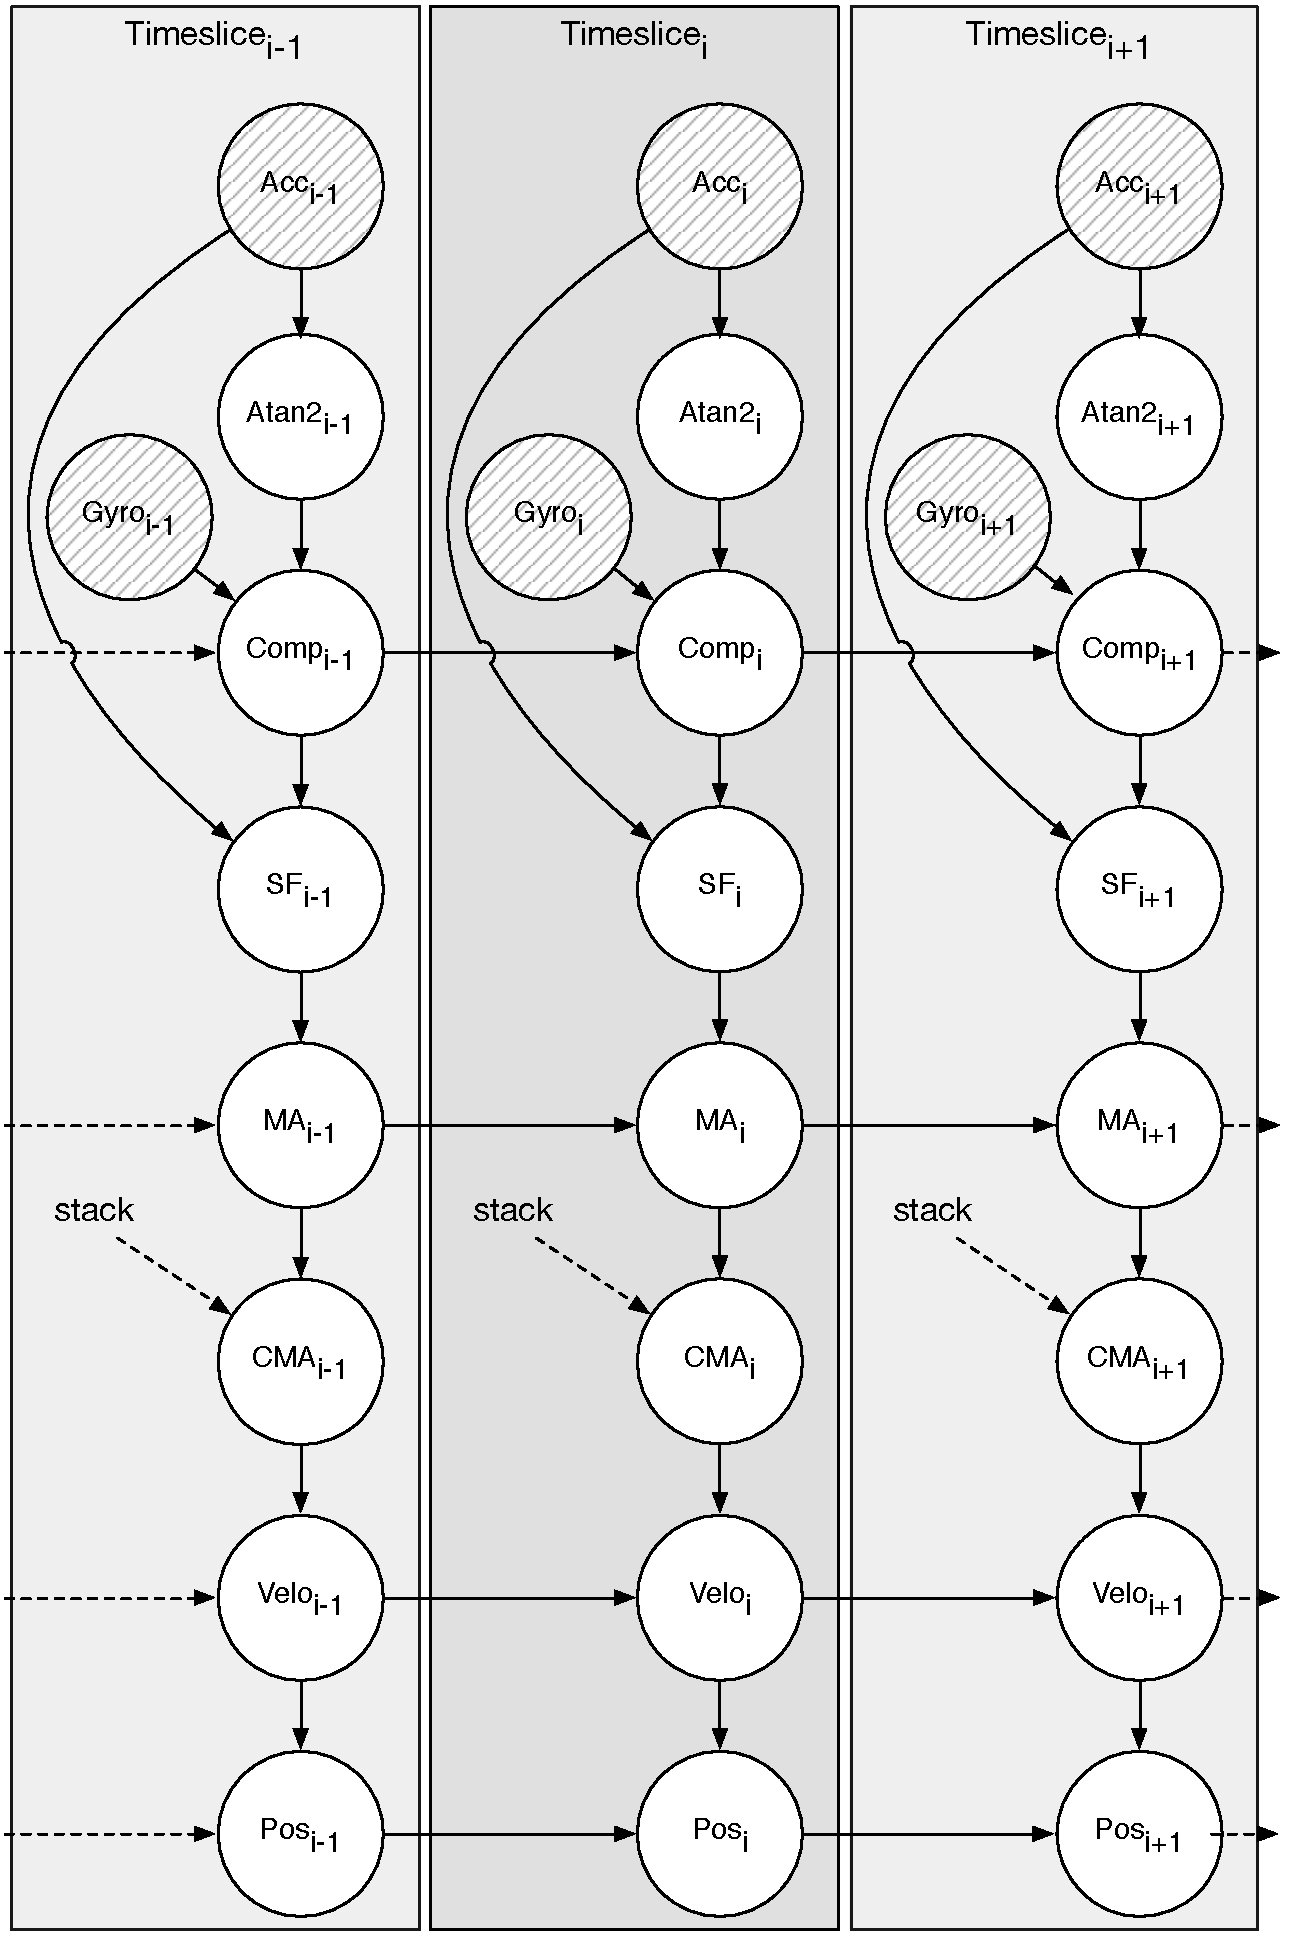
\includegraphics[scale=0.6]{media/dynamic-bayesian-network}
\caption{Dynamic Bayesian Network}
\label{figure:dynamic-bayesian-network}
\end{figure}

To make sure, every acceleration is followed by an equal deceleration, the \textit{CMA}, short for Corrected Moving Average, variable is implemented.
The purpose of CMA is to save MA variables in a stack, so that once deceleration begins, the application will pop elements from the stack and use these values negated.

The \textit{Velo} variable calculates the current velocity by using the values obtained from the CMA and previous Velo variables. 
Lastly, the \textit{Pos} variable calculates a new position, by looking at the previous Pos and the current Velo variable.

Probability distributions will be determined as described in \secref{section:normal-distribution}.
The structure of the dynamic Bayesian network is based on the physical laws for the relation between acceleration, velocity, and position, as described in \secref{sec:position-calculations}.
%\section{Probability}\label{section:probability}
This section is regarding probability, specifically forward propagation.
The concept of probability in machine intelligence is to make a decision based on observations of a domain.
The information, which is used for calculating probability can be discrete or continuous. 
In this project the primary focus will be on continuous variables, however discrete variables will be briefly explained.

\subsection{Discrete Variables}\label{subsection:discrete-variables}
In probability, $\Omega$ is used to describe the set of possible worlds, which contains all the states or variables in that space, e.g. all the possible numbers a dice can roll $(\Omega = \{1, 2, 3, 4, 5, 6\})$, which is a finite set.
The probability space, written $P(a)$, is the probability of some variable or event, e.g. the probability of rolling even numbers with a dice $P(even = true) = P(2) + P(4) + P(6) = 3/6$. 
There can be a proposition for an event, where the proposition can either be true or false, e.g a six-sided dice can have the following proposition:
$$P(dice) = one_{eye} \vee two_{eye} \vee three_{eye} \vee four_{eye} \vee five_{eye} \vee six_{eye}$$
It is possible to find the probability of an event given that another event has occurred, which have an effect on the state space.
It is called conditional probability and is denoted by $P(A|B)$ which can be translated as \textit{the probability of A given B}.
Sometimes these event are independent meaning that they do not affect each other, e.g. the outcome of a new roll, is not affected by the previous roll.
To find the probability distribution, the 
Gaussian distribution is used to find the probability around a given point.
The distribution can be used to find the probability between two numbers by integrating the Gaussian distribution function.

\subsection{Continuous Variables}\label{subsection:continuous-variables}
The properties of continuous variables are described in \secref{section:bayesian-network}.
Probability for continuous variables is different from discrete variables, as the set of possible worlds $\Omega$ = $\{\mathbb{R}\}$, which is not a finite set. 
The probability for a continuous random variable X can be written as $P(a \leq X \leq b)$, where a and b are exact numbers.
The probability can be calculated in different ways, one of which is a probability density function.

For continuous variables the continuous probability density function can be calculated by taking the integral of the density function. 
It is defined as:
\begin{equation}
\int\limits_{a}^{b} f(x)dx 
\end{equation}
where $a$ and $b$ determines the interval of the integral. 
If $a = -\infty$ and $b = \infty$, the integral of the graph will have a probability of 1.

A simple example for using continuous variables is finding the probability for the amount of rain that will fall tomorrow, $P(Y)$. 
A function for the rain fallen, $f(x)$, could be shown as in \figref{figure:pdf-graph}.
The probability for this could be described as an interval:
$P(1.5 \le Y \le 2.5)$

From the graph, it can be seen that the probability of the amount of rain, that will fall tomorrow, is more likely to be between numbers 1.5 and 2.5 rather than between 3 and 4.
The exact probability for this can be found by using the integral of function $f(x)$:
$\int\limits_{1.5}^{2.5} f(x)dx$.

\begin{figure}[h]
	\centering
	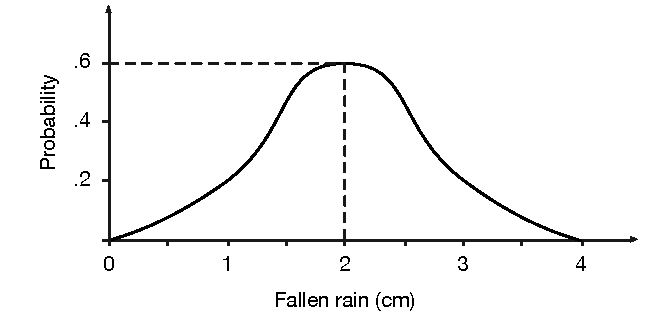
\includegraphics[scale = 0.7]{media/Theory/probability-density-function}
	\caption{A probability distribution over how much rain has fallen.}
	\label{figure:pdf-graph}
\end{figure}
\section{Normal Distribution}\label{section:normal-distribution}
In this section, the theory needed to use normal distributions is presented and explained, and has primarily been based on \citet{article:Lauritzen, article:thiesson}.

A normal distribution is common when working with continuous variables \citep{misc:artificial-intelligence}. 
It is a distribution that can be specified by giving the mean and variance, the uncertainty about the expected value of the distribution, notated as $\mathcal{N}(\mu, \sigma^2)$. 
It could be a distribution for the expected result of i.e. acceleration, velocity, or position.

The theory of univariate and multivariate normal distributions is described hereafter, where univariate is for a variable influenced by one factor, whereas multivariate is by multiple factors. 

\subsection{Univariate}
The actual function for a univariate normal distribution is as follows:

\begin{equation}\label{eq:normaldist}
	f(x) = \frac{1}{\sigma \sqrt{2\pi}}e^{-\frac{(x - \mu)^2}{2 * \sigma^2}}
\end{equation}
where, 
\begin{itemize}
	\item[$\mu$] is the mean value of the data. It gives the position of the normal distribution, which is approximated by using $\mu = \frac{1}{n}\sum\limits_{n}\left(X_n\right)	$.
	\item[$\sigma$] is the standard deviation. It is a measurement for the variance of the data, and determines how flat the normal distribution is. $\sigma ^2$ is the variance that is approximated by using $\sigma^2 = \frac{1}{n}\sum\limits_{n}\left( X_n - \mu \right)^2$.
\end{itemize}

\begin{figure}[h]
	\centering
	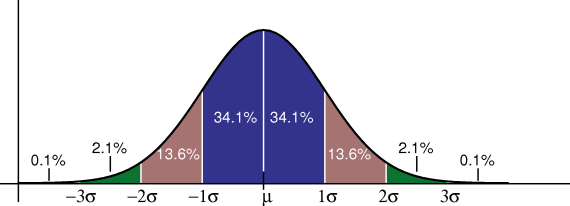
\includegraphics[scale=2]{media/Theory/stddev}
	\caption{Normal distribution \citep{book:gaussian}.}
	\label{fig:stddev}
\end{figure}

To have an idea of how a normal distribution looks, see \figref{fig:stddev}. The figure indicates how the probability is distributed around $\mu$, where $68\%$ of the values is in the range of $\mu \pm \sigma$.
If the integral is taken from $-\infty$ to $\infty$, it will result in $100\%$.

\subsection{Multivariate}
To update the probability distributions for the given variables in the Bayesian network, for each timeslice, it is necessary to have some general theory for joining and marginalisations of probabilities.

The probability distribution for a stochastic vector $X$, where the distribution is normal and not affected by other variable distributions, is defined as follows.
\begin{equation}\label{eq:normaldistindependent}
p(X)=\mathcal{N}(A, C)
\end{equation}

As can be seen in \eqref{eq:normaldistindependent}, the mean value is solely based on $A$, which is a $\begin{bmatrix}a \times b\end{bmatrix}$ matrix.
%For acceleration  in this project it would be the recorded acceleration value, since for acceleration in 1 axis $a = 1$. 
Furthermore, $C$ is a $\begin{bmatrix}a \times a\end{bmatrix}$ co-variance matrix for the normal distribution of $X$. 

When a stochastic vector $Y$ is affected by another stochastic vector $X$, then the conditional density for $Y$ given $X$ is defined as follows. 
\begin{equation}\label{eq:normaldistaffected}
p(Y|X)=\mathcal{N}(E + F * A, G)
\end{equation}

In \eqref{eq:normaldistaffected}, $E + F * A$ can be seen and is a linear regression on $A$.
$E$ is a $\begin{bmatrix}1 \times d\end{bmatrix}$ gain matrix that can be defined, for example if there is a tendency to get a mean value that is always $0.1$ lower than the actual value, $E$ could be $0.1$ to take this into account.
$A$ is a $\begin{bmatrix}c \times d \end{bmatrix}$ matrix, containing the mean values of the parent variables of the affected variable, where $Y$ is the child.
$F$ in this case is a $\begin{bmatrix}1 \times c\end{bmatrix}$ matrix, and is defined such that it correctly describes how $X$ affects the mean value for $Y$, which varies depending on how $X$ is constructed. 
That is, how the different elements of $A$, which are based on the mean values of $X$, affect the mean value of $Y$.
$G$ is the cardinal covariance matrix, for $Y$ given $X$, which for this project has not been determined accurately.
Utilising machine learning techniques, could be helpful to determine the accurate $G$. 

\subsection{Direct Combination}\label{section:direct-combination}
The equation to calculate the joint distribution of $Y$ and $X$ is as follows:
\begin{equation}\label{eq:jointdist}
\begin{aligned}
P(Y,X)&=P(Y|X)*P(X)=\mathcal{N}(U+V,W)\\
U&= 
\begin{bmatrix}
\mu_X \\
\mu_Y 
\end{bmatrix}
= \begin{bmatrix}
A \\
E + F * A
\end{bmatrix}\\
V &= 0\\
W &=
\begin{bmatrix}
\Sigma_{XX} & \Sigma_{XY} \\
\Sigma_{YX} & \Sigma_{YY}
\end{bmatrix}
=
\begin{bmatrix}
C & C * F^\intercal \\
F*C & G + F * C * F^\intercal
\end{bmatrix}
\end{aligned}
\end{equation}

As can be seen in \eqref{eq:jointdist}, $U$ consist of the mean values of $X$ and $Y$.
When $P(X)$ and $P(Y|X)$ have been defined, the partial result can directly be used for $U$.
No additional gain other than $U$ is relevant since $V=0$, as there are no conditional variables in $P(Y,X)$.
The covariance matrix $W$ for $P(Y,X)$ can, as $U$, also be constructed by the partial results of marginalisation $X$ in $P(X)*P(Y|X)$.
The elements of $W$ consists of the variance of $X$ and $Y$ on the diagonal, where the other elements are the co-variances of $X$ and $Y$ combined.
In order to calculate the probability distribution for $Y$, \eqref{eq:marginalised} is used.
\begin{equation}\label{eq:marginalised}
P(Y)=\mathcal{N}(E+F*A,G+F*C*F^\intercal)
\end{equation}

\eqref{eq:marginalised} has been constructed by using $P(Y,X)$, where $X$ has been marginalised out. 
Since the probability distribution, which is being worked with, is a normal distribution, this
marginalisation becomes trivial.
The mean value in the equation is $E+F*A$, since it is the $Y$ part of $U$ in \eqref{eq:jointdist}.
The variance is element $(2,2)$ in $W$ from \eqref{eq:jointdist}.

\subsection{Insertion of Evidence}\label{section:insert-evidence}
When able to calculate the joint distribution of two stochastic variables, it is possible to update the probability distributions with insertion of evidence, which is defined as follows.

\begin{equation}\label{eq:evidence}
\begin{aligned}
P(Y,E) &= \mathcal{N}\left(\begin{bmatrix} A_Y \\ A_E\end{bmatrix}, \begin{bmatrix}C_{YY} & C_{YE} \\ C_{EY} & C_{EE}\end{bmatrix}\right) \\
P(Y,E=e) &= \mathcal{N}\left(U,W\right) \\
U &= A_Y + C_{YE} * (e - A_E) * C_{EE}^{-1} \\
W &= C_{YY} - C_{YE} * C_{EY} * C_{EE}^{-1}
\end{aligned}
\end{equation}

As can be seen in \eqref{eq:evidence}, when evidence is inserted for a stochastic variable, the joint distribution for two variables where one of them has evidence inserted, can be determined from the evidence and the joint distribution of these two variables.

The insertion of evidence theory described above works when having an exact observation. 
However, if an observation is uncertain, the above formulas do not work since the variance from the observation wont have effect on the marginalised distribution of the parent node of the observation.
The theory for evidence can, however, be used in other settings such as the Kalman filter, since in that case the observation is certain.

\subsection{Applying the Formulas}
With the general theory for direct combination described, applying the theory to the Bayesian network for this project can be performed.

See \eqref{eq:accdist} for an example of how to determine the normal distribution of the acceleration.
\begin{equation}\label{eq:accdist}
P(acc_{i+1})=\mathcal{N}(acc_{i+1},\sigma^2_{acc})
\end{equation}

\eqref{eq:accdist} consists of $acc_{i+1}$, which is the recorded data from the accelerometer, and $\sigma^2_{acc}$ is the variance, which is determined in \secref{section:finding-the-variance}. 
The reason the acceleration is represented as a single stochastic node and not as two nodes, where one is the observation of the acceleration and the other is the actual acceleration, is as follows.
As discussed in the previous section about evidence, the variance for the observation would not have an impact on the actual acceleration node. 
For that reason, acceleration has been modelled as a single stochastic node to take the acceleration variance into account for its descendants.

Once this normal distribution is determined, the normal distribution for the moving average of the acceleration $MA_{i+1}$, as seen in \figref{fig:direct-combination}, can be found.

\begin{figure}[H]
\centering
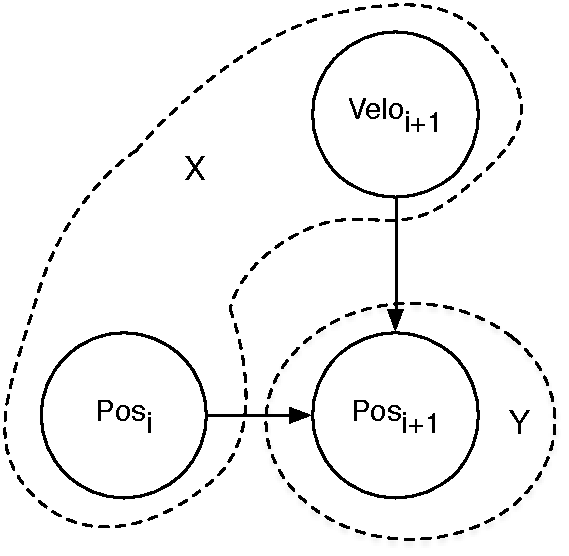
\includegraphics[scale=0.4]{direct-combination}
\caption{A family, or segment, of the Bayesian network from \secref{section:dynamic-bayesian-network}.}
\label{fig:direct-combination}
\end{figure}

With the assumption of a Bayesian network as in \figref{fig:direct-combination}, \eqref{eq:probabilityformovingaverage} is valid, given the previous theory.
\begin{equation}\label{eq:probabilityformovingaverage}
\begin{aligned}
P(Pos_{i+1})&=\mathcal{N}(F_{Pos}*A_{Pos_{i+1}},G_{Pos_{i+1}}+F_{Pos}*C_{Pos_{i+1}}*{F_{Pos}}^\intercal)\\
\text{where}&\\
F_{Pos}&=\begin{bmatrix} \Delta t & 1\end{bmatrix}\\
A_{Pos_{i+1}}&=\begin{bmatrix} \mu(Velo_{i+1}) \\ \mu(Pos_i)\end{bmatrix}\\	
C_{Pos_{i+1}}&=\begin{bmatrix} var(Velo_{i+1}) & 0 \\ 0 & var(Pos_{i}) \end{bmatrix}\\
\end{aligned}
\end{equation}

In \eqref{eq:probabilityformovingaverage}, $F_{Pos}$ is based on the formula for exponential moving average, as seen in \subsecref{subsection:exponential-moving-average}.
$A_{Pos}$ is based on the mean values for the parent variables of $Pos_{i+1}$.
$C$ is a $\begin{bmatrix}2 \times 2\end{bmatrix}$ matrix and is constructed from the variance of the parents.
$G_{Pos_{i+1}}$ is a cardinal covariance matrix for $Pos_{i+1}$ given a stochastic vector consisting of $Velo_{i+1}$ and $Pos_i$.


For a complete set of formulas for the Bayesian network in \secref{section:dynamic-bayesian-network}, derived from the theory in this section, see \appref{app:direct-combination}.
The formulas are excluded from this section as they are derived similar to \eqref{eq:probabilityformovingaverage}.

In principle, to propagate through a family, the process is to first calculate the marginal and conditional distributions and then make a joint distributions for these, whereafter a marginal distribution for the child is found.
\section{Game Design}\label{section:game-design}
The intended design of the game will be similar to \textit{Squash}, while retaining the graphics of \textit{Pong}. 
In \figref{figure:game-layout} the layout of the game board can be seen. 
The basic elements of the game are the ball, the paddle, the walls, and power-ups. 
The main objective of the game is to prevent the ball from moving past the paddle.

\begin{figure}[h]
	\centering
	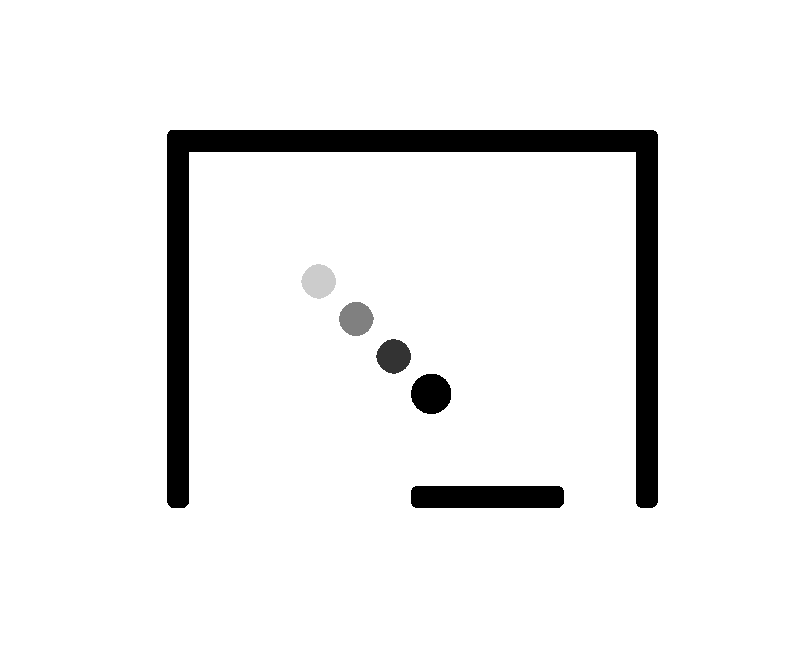
\includegraphics[scale = 0.3]{media/design/game-layout.pdf}
	\caption{The layout of the game board}
	\label{figure:game-layout}
\end{figure}

An important game design aspect is the control of the paddle, which in this project relies on dead reckoning for movement tracking. 
It means if the player moves left or right, the paddle will follow his movements. 

While the basic elements of the game are simple, some additional features have been added to the game to enhance the user experience.
Some of these features include a scoring system and power-ups.
The score is based on the time the player keeps the game alive, meaning as long as there is at least one ball on the board, the score increases.
Power-ups could increase the size of the paddle, get an extra ball on the board, or slow the speed of the balls, and negative power-ups could decrease the paddle size, increase the speed of the balls, or decrease the score.
A story board of how the game should work can be seen in \figref{figure:story-board}.
\begin{figure}[H]
	\centering
	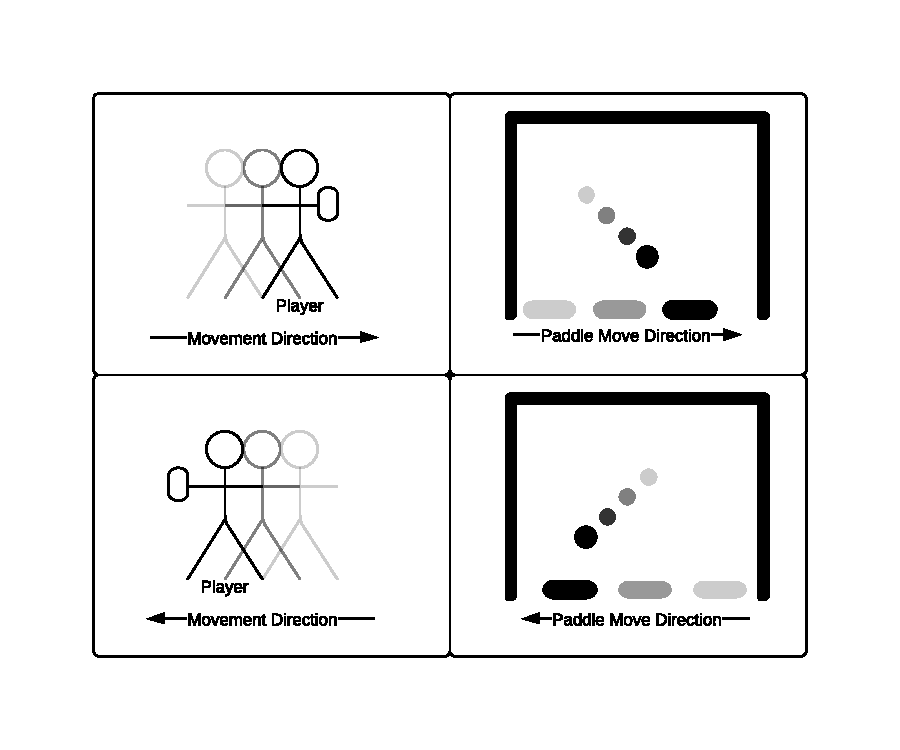
\includegraphics[trim = 0cm 1.5cm 0cm 1.5cm, clip, scale = 0.75]{media/design/story-board.pdf}
	\caption{A storyboard of how the game is played}
	\label{figure:story-board}
\end{figure}

%FEATURES
%POWERUP: BIGGER PADDLE, MOAR BAALS, SLOW ALL BALLS, DOUBLE POINTS FOR x TIME, 
%NEGATIVE POWERUPS: SMALLER PADDLE, FASTER BAAALS, FLASHING BALLS, -x\% score, inverted controls
%HIGHSCORE


\section{Events}\label{section:event-table}
The event table in \tabref{table:event-table} represents the possible events in the game and how they are connected to the classes.
The classes used are \textit{Paddle}, \textit{Ball}, \textit{Time}, and \textit{Score}.
The Paddle class ensures that the movements of the player corresponds to the paddle in the game.
The Ball class represents the ball which moves on the board, and can bounce off the walls and the paddle. 
Time starts when the game starts and stops when the ball is not caught.
Time is also used to limit the duration of power-ups and increases the score as time passes.

\begin{table}[h]
\centering
\begin{tabular}{| c | c | c | c | c |}
\hline
 & Paddle & Ball & Time & Score \\\hline
Lose game & & + & + & + \\ \hline
Move & * & & & \\ \hline 
Spawn ball & & + & &  \\\hline
Despawn ball & & + & &  \\\hline
Spawn power-up & & & * & \\\hline
Change paddle size  & * & & & \\\hline
Increase ball speed & & * & * & \\\hline
Decrease ball speed & & * & & \\\hline
Increase score & & & * & *\\\hline
Score multiplier & & & & * \\\hline
\end{tabular}
\caption{Event Table, * meaning zero to many and + meaning zero to one.}
\label{table:event-table}
\end{table}

\textit{Lose game} is an event that happens when the ball is not caught by the paddle. 
When the event occurs, the time is stopped and the Score is saved in case the user wants to submit it to the high score.
To avoid losing the game, the paddle has to be able to move.
The \textit{Move} event works together with dead reckoning to get the movement of the player, and enables the paddle to move left and right.

\textit{Spawn power-up} is an event that spawns a power-up in the game, which occurs randomly after some time.
One of the power-ups that can spawn is a power-up that increases the paddle size and the counterparting power-up decreases the paddle size.

The ball spawns when the game starts, and despawns when the ball is not caught.
This is handled by the \textit{Spawn ball} and \textit{Despawn ball} events.
The ball speed is increased over time, but can also be changed with the help of power-ups, which is the \textit{Increase ball speed} and \textit{Decrease ball speed} event.

The score can be affected by two different events.
\textit{Increase score} happens over time, whereas \textit{Score multiplier} occurs when its corresponding power-up is caught, resulting in either a doubling or halving of the score, depending on the power-ups colour.

\section{State Diagram}\label{section:state-diagram}

A state diagram shows the different states the program can be in and the options the user can perform to change the state of the program.
State diagrams are useful models for designing the interfaces. 
The state diagram for this project can be seen in \figref{figure:state-diagram}, which includes all the transitions and states for the program. 

\begin{figure}[h]
	\centering
	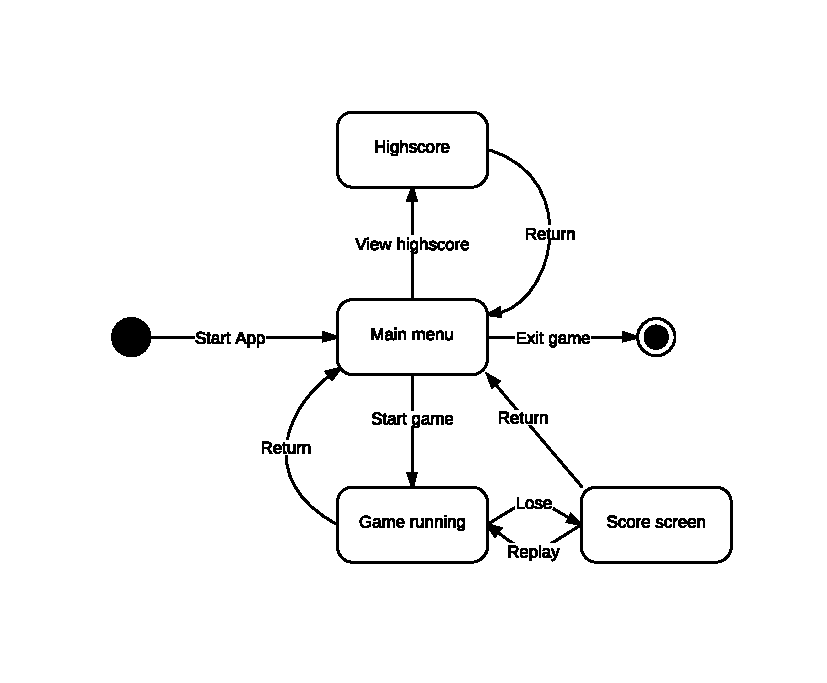
\includegraphics[trim = 0cm 1.5cm 0cm 1.5cm, clip, scale = 1]{media/design/state-diagram.pdf}
	\caption{Application state diagram.}
	\label{figure:state-diagram}
\end{figure}

Initially, the user will launch the application, which will present the \textit{Main menu}.
From here, the user can press the buttons \textit{Start game}, \textit{View highscore}, or \textit{Exit game}. 
Start game will render the game to begin, and the application will now be in the state \textit{Game running}, it will remain in this state until the user loses the game, or the user chooses to \textit{Return} to the Main menu.
When the user loses the game, a \textit{Score screen} will appear, allowing the user to \textit{Replay} or Return to the Main menu. 
Furthermore, when a user loses a game, the achieved score can be submitted to the highscore, which can be viewed in the \textit{Highscore} state.
The Highscore state can be accessed from the Main menu.
\section{Concepts}\label{section:prototype}
In this section concepts will be illustrated. 
The concepts will be used as a draft before implementing the final application, where the state diagram \figref{figure:state-diagram} is used to derive the layout.

The user is first presented with the \textit{Main Menu}, which can be seen in \figref{figure:main-menu}.
The Main Menu will enable the user to start the game and view the \textit{High score}.
In the High score, \figref{figure:highscore}, the user can see a list of scores achieved on the phone.

\begin{figure}[H]
	\centering
	\begin{subfigure}[b]{0.3\textwidth}
	
\includegraphics[scale = 0.55]{media/prototype/main-menu.png}
	\caption{Main Menu}
	\label{figure:main-menu}
	\end{subfigure}
	\qquad
	\begin{subfigure}[b]{0.3\textwidth}
	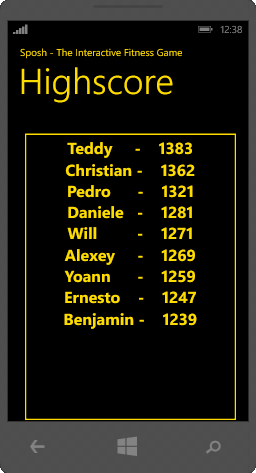
\includegraphics[scale = 0.55]{media/prototype/highscore.png}
	\caption{High score}
	\label{figure:highscore}
	\end{subfigure}
	\caption{The prototype of the Main Menu(\textit{a}) and the High score (\textit{b})}
\end{figure}
In \figref{figure:thegame}, the user plays the game. 
In this screen the borders of the game, the ball, and the paddle can be seen.
When the ball has passed the paddle, the user loses the game and is taken to the score screen, where the user can save his score, replay the game, or return to the main menu, as can be seen in \figref{figure:score-screen}.

\begin{figure}[H]
	\centering
	\begin{subfigure}[b]{0.4\textwidth}
	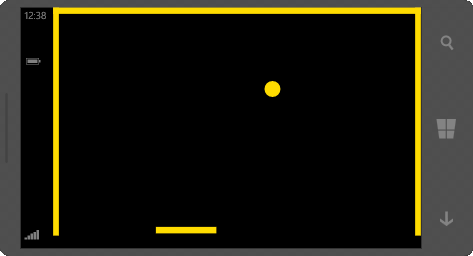
\includegraphics[scale = 0.5]{media/prototype/game.png}
	\caption{The Game.}
	\label{figure:thegame}
	\end{subfigure}
	\qquad
	\begin{subfigure}[b]{0.4\textwidth}
	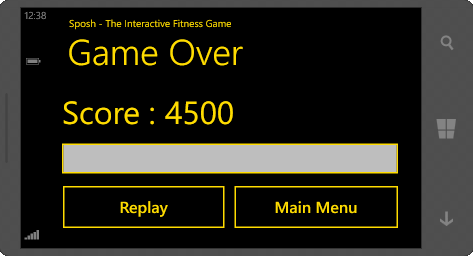
\includegraphics[scale = 0.5]{media/prototype/score-screen.png}
	\caption{The Score Screen.}
	\label{figure:score-screen}
	\end{subfigure}
	\caption{The game (\textit{a}) and the score screen (\textit{b})}
\end{figure}

